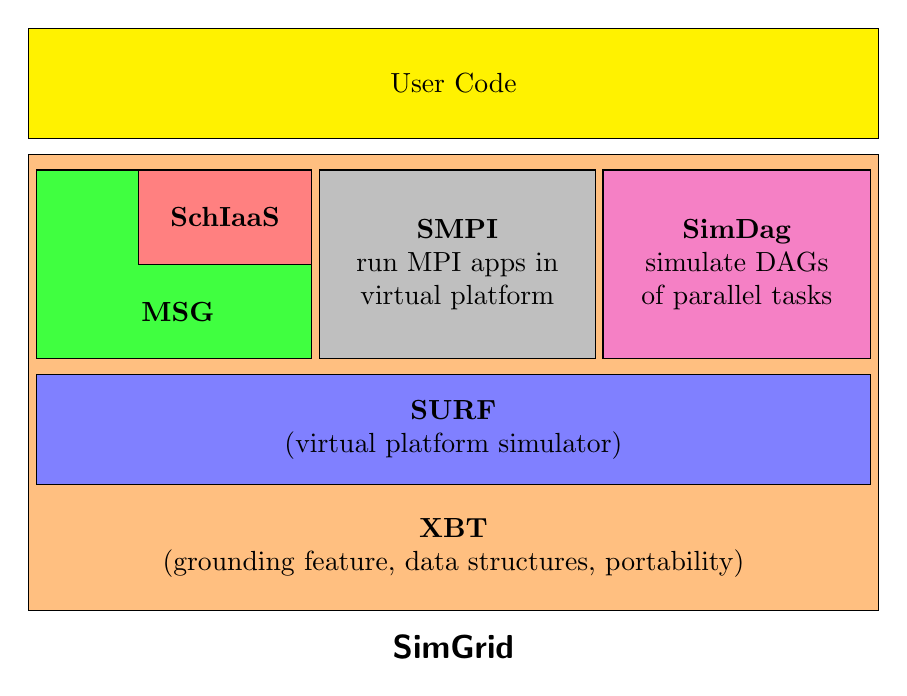
\begin{tikzpicture}[x=1cm,
y=1cm,
every node/.style={
rectangle,
align = center,
anchor=south west,
outer sep=1mm,
},
box/.style={
draw,
}]

%Simgrid box
\node[box,minimum height=5.8cm,minimum width=10.8cm,fill=orange!50,label={south:\large{}\textsf{\textbf{SimGrid}}}]at(0,0){};
%\node[box,minimum height=5.8cm,minimum width=1.4cm,fill=cyan!50]at(11,0){\rotatebox{270}{\textbf{Tracing}}};
\node[minimum height=1.4cm,minimum width=10.6cm]at(0.1,0.1){\textbf{XBT}\\(grounding feature, data structures, portability)};
\node[box,minimum height=1.4cm,minimum width=10.6cm,fill=blue!50]at(0.1,1.6){\textbf{SURF}\\(virtual platform simulator)};
\node[box,minimum height=2.4cm,minimum width=3.5cm,fill=green!75]at(0.1,3.2){};
\node[box,minimum height=2.4cm,minimum width=3.5cm,fill=gray!50]at(3.7,3.2){\textbf{SMPI}\\run MPI apps in\\ virtual platform};
\node[box,minimum height=2.4cm,minimum width=3.4cm,fill=magenta!50]at(7.3,3.2){\textbf{SimDag}\\simulate DAGs\\ of parallel tasks};

\node[box,minimum height=1.2cm,minimum width=2.2cm,fill=red!50]at(1.4,4.4){\textbf{SchIaaS}};
\node[minimum height=1.2cm,anchor=south]at(2,3.2){\textbf{MSG}};

\node[box,minimum height=1.4cm,minimum width=10.8cm,fill=yellow]at(0,6){User Code};
\end{tikzpicture}